% Copyright 2004 by Till Tantau <tantau@users.sourceforge.net>.
%
% In principle, this file can be redistributed and/or modified under
% the terms of the GNU Public License, version 2.
%
% However, this file is supposed to be a template to be modified
% for your own needs. For this reason, if you use this file as a
% template and not specifically distribute it as part of a another
% package/program, I grant the extra permission to freely copy and
% modify this file as you see fit and even to delete this copyright
% notice. 

\documentclass{beamer}
\mode<presentation> {
% There are many different themes available for Beamer. A comprehensive
% list with examples is given here:
% http://deic.uab.es/~iblanes/beamer_gallery/index_by_theme.html
% You can uncomment the themes below if you would like to use a different
% one:
%\usetheme{AnnArbor}
%\usetheme{Antibes}
%\usetheme{Bergen}
%\usetheme{Berkeley}
%\usetheme{Berlin}
%\usetheme{Boadilla}
%\usetheme{boxes}
%\usetheme{CambridgeUS}
\usetheme{Copenhagen} %****
%\usetheme{Darmstadt}
%\usetheme{default}
%\usetheme{Frankfurt}
%\usetheme{Goettingen}
%\usetheme{Hannover}
%\usetheme{Ilmenau}
%\usetheme{JuanLesPins}
%\usetheme{Luebeck}
%\usetheme{Madrid}
%\usetheme{Malmoe}
%\usetheme{Marburg}
%\usetheme{Montpellier}
%\usetheme{PaloAlto}
%\usetheme{Pittsburgh}
%\usetheme{Rochester}
%\usetheme{Singapore}
%\usetheme{Szeged}
%\usetheme{Warsaw}
}

\usepackage{graphicx} 
\usepackage{booktabs} 
\usepackage[portuguese]{babel}
\usepackage[utf8]{inputenc}
\usepackage{multicol}
\usepackage{blindtext}

\title{Análise Comparativa de Modelos Para Dados Longitudinais no Estudo da Contagem do Número de Bactérias
       Presentes no Leite de Vaca}

% A subtitle is optional and this may be deleted
%\subtitle{Teoria }

\author{Alexandre Diaz \and Simone Matsubara \and Willian Meira}
% - Give the names in the same order as the appear in the paper.
% - Use the \inst{?} command only if the authors have different
%   affiliation.

\institute[UFPR] % (optional, but mostly needed)
{
  Disciplina Análise de Dados Longitudinais \\
  Professor José Padilha\\
  Departmento de Estatística - UFPR
  }
% - Use the \inst command only if there are several affiliations.
% - Keep it simple, no one is interested in your street address.

\date{\today}

%\subject{Theoretical Computer Science}

\AtBeginSubsection[]
{
  \begin{frame}<beamer>{Índice}
    \tableofcontents[currentsection,currentsubsection]
  \end{frame}
}

% Let's get started
\begin{document}

%---------------------------
\begin{frame}
\titlepage % Print the title page as the first slide
\end{frame}
%---------------------------

%---------------------------
\begin{frame}{Autores}
    \begin{itemize}
        \item Idemauro Antonio Rodrigues de Lara
          \begin{itemize}
            %\item ESALQ/USP - Depto de Ciências Exatas
            \item Universidade de São Paulo – USP, Escola Superior de Agricultura Luiz de Queiroz - ESALQ,                           Departamento de Ciências Exatas
          \end{itemize}
        \item Maria Helena Constantino Spyrides 
          \begin{itemize}
            \item Universidade Federal do Rio Grande do Norte – UFRN, Departamento de Estatı́stica
          \end{itemize}   
        \item Mirela Gurgel
          \begin{itemize}
            \item Unidade Acadêmica Especializada em Ciências Agrárias
          \end{itemize}
        \item Adriano Henrique do Nascimento Rangel
          \begin{itemize}
            \item Unidade Acadêmica Especializada em Ciências Agrárias
          \end{itemize} 
    \end{itemize} 
\end{frame}

%---------------------------
%---------------------------
\begin{frame}
  \frametitle{Estudo Longitudinal} % Table of contents slide, comment this block out to remove it
  \tableofcontents % Throughout your presentation, if you choose to use \section{} and \subsection{} commands,       these will automatically be printed on this slide as an overview of your presentation
\end{frame}

%----------------------------------------------------------------------------------------
%	PRESENTATION SLIDES
%----------------------------------------------------------------------------------------

%------------------------------------------------
%\section{Sumário} % Sections can be created in order to organize your presentation into discrete blocks, all sections and subsections are automatically printed in the table of contents as an overview of the talk
%------------------------------------------------
% OK *********************************************************************************

\subsection{Motivação}
    \begin{frame}{Motivação}
        \begin{block}{}
            Identificar covariáveis ou fatores que mais contribuem para o aumento da Contagem Bacteriana 
            Total (CBT) no leite de vaca a fim de avaliar os impactos dos procedimentos de manejo, na 
            ordenha, limpeza de equipamentos e do tanque de resfriamento sob essa variável durante o 
            processo de produção do leite para ações corretivas.
        \end{block}
    \end{frame}
%------------------------------------------------

\subsection{Introdução}
    \begin{frame}{Introdução}
        \begin{itemize}
          \item A contagem bacteriana total (CBT) no leite cru - análise de qualidade        
          \item Condições inadequadas favorecem a proliferação de bactérias
          \item Órgão regulador: Ministério da Agricultura, Pecuária e Abastecimento (MAPA)
          \item Instrução Normativa nº 51/2002
            \begin{itemize}
              \item Limite de 750.000 ufc/mL
              \item A partir de 2012: 100.000 ufc/mL
              \item 50\% das amostras coletadas ficaram acima do limite estabelecido
            \end{itemize}
        \end{itemize}
    \end{frame}
% OK *********************************************************************************

\subsection{Metodologia}
    \begin{frame}{Metodologia}
         \begin{itemize}
            \item Estudo conduzido em 8 propriedades localizadas no RN
            \item Foram coletadas 4 medidas repetidas mensalmente em cada propriedade
            \item Realizado entre jan/2010 a jul/2011 e dividido em 3 períodos:
              \begin{itemize}
                \item Diagnóstico: de janeiro a abril de 2010
                \item Capacitação: de maio a dezembro de 2010
                \item Acompanhamento: de janeiro a julho de 2011
              \end{itemize} 
         \end{itemize} 
     \end{frame}
     
     \begin{frame}{Metodologia - Fatores avaliados}
        \begin{block}{}
          Foram levados em consideração diversos fatores importantes no manejo da ordenha. Estes fatores foram divididos em 3 categorias
        \end{block}
     
     
         \begin{itemize}
                \item 1) Ordenha: teste da caneca, pré-dipping e secagem com papel toalha
                \item 2) Limpeza 1 (ordenha): sanitização, limpeza alcalina e ácida
                \item 3) Limpeza 2 (tanque): resfriamento, sanitização, limpeza
         \end{itemize} 
     \end{frame}

    \begin{frame}{Metodologia - Modelos Ajustados}
        %\textbf{Objetivos}
         \begin{itemize}
            
            \item Modelo Marginal Poisson
            \begin{block}{}
                    \eta_i_t = ln(\mu_i_t) = \beta_0 + \beta_1_jper_j + \beta_2ord + \beta_3limp1 + \beta_4limp2
            \end{block}

            \item Modelo Misto (efeito aleatório)
              \begin{block}{}
                    \eta_i_t = (\beta_0 + b_i_0) + (\beta_1_j + b_i_1_j)per_j + \beta_2ord + \beta_3limp1 + \beta_4limp2
              \end{block}

        \end{itemize} 
 
     \end{frame}


% OK *********************************************************************************
% OK *********************************************************************************
\subsection{Resultados e Discussão}
    \begin{frame}{Estatísticas descritivas - Contagem bacteriana total}
        \begin{figure}[!h]
            \centering
            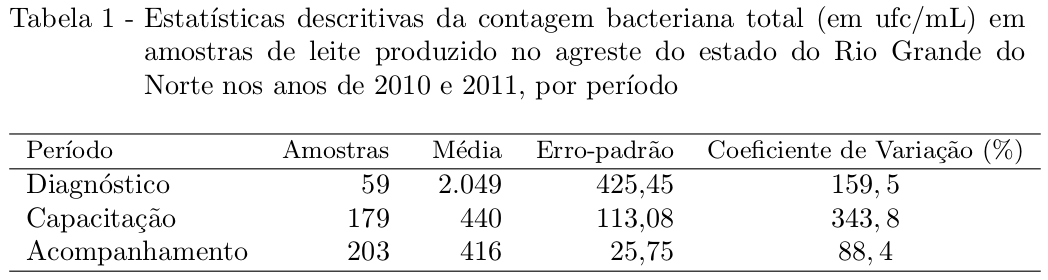
\includegraphics[scale=0.29]{long_tab01.png}
            %\caption{}
            \label{Rotulo}
        \end{figure}
    \end{frame}

    \begin{frame}{Estatísticas descritivas - Adequação das propriedades à IN51}
        \begin{figure}[!h]
            \centering
            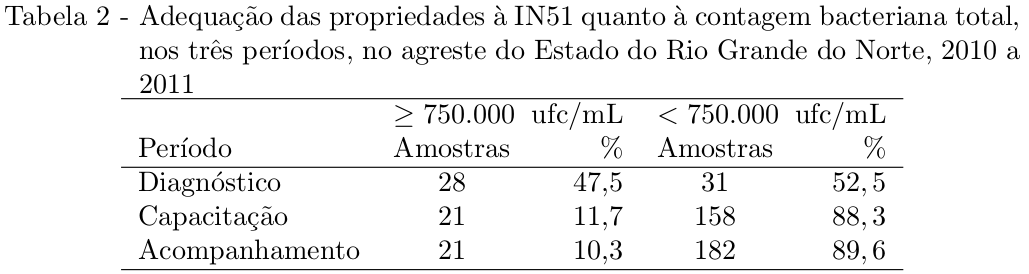
\includegraphics[scale=0.30]{long_tab02.png}
            %\caption{}
            \label{Rotulo}
        \end{figure}
    \end{frame}

    \begin{frame}{Perfis individuais de CBT}
        \begin{figure}[!h]
            \centering
            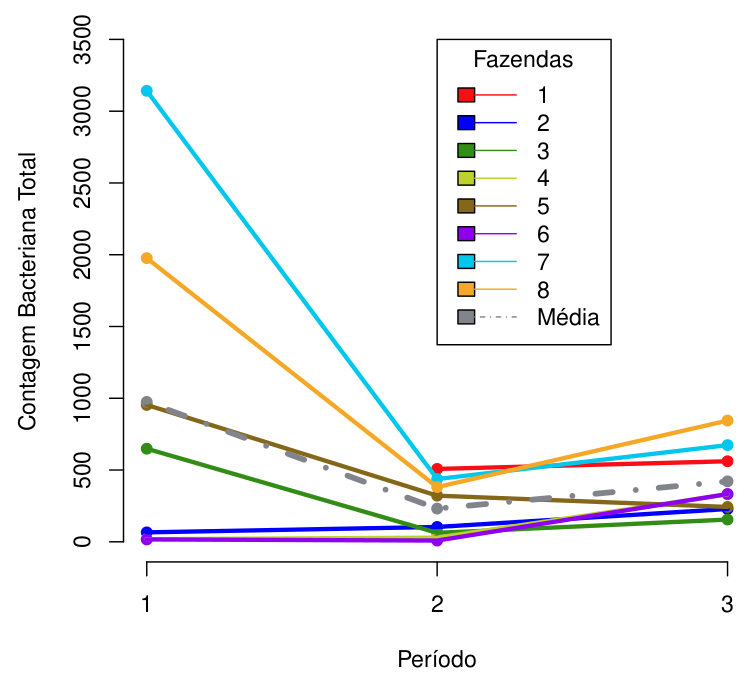
\includegraphics[scale=0.25]{long_graf01.png}
            %\caption{}
            \label{Rotulo}
        \end{figure}
    \end{frame}

   \begin{frame}{Estrutura de correlação}
        \begin{block}{}
          Estruturas de correlação testadas: Simetria Composta, m-Dependente, Não-Estruturada e Auto-Regressiva (AR).
        \end{block}
        
        \begin{figure}[!h]
            \centering
            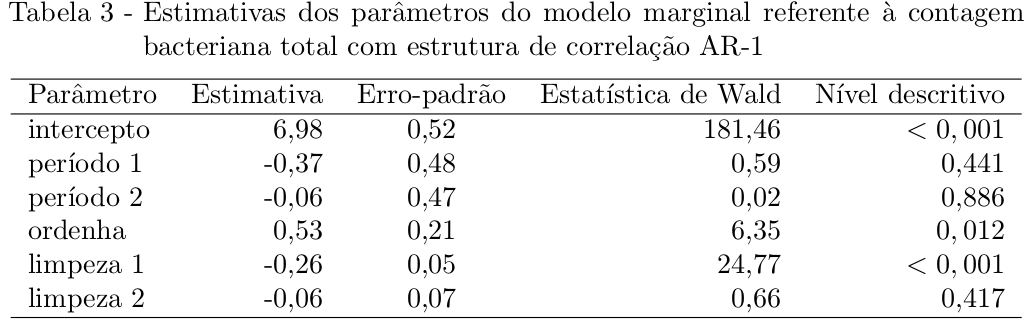
\includegraphics[scale=0.29]{long_tab03.png}
            %\caption{}
            \label{Rotulo}
        \end{figure}
 
 \end{frame}

\begin{frame}{Estrutura de correlação - Interpretação}
  \begin{itemize}
    \item Efeitos referente à ordenha e limpeza 1 são significativos a 5\%. 
    \item Quanto maior o número de procedimentos realizados nas covariáveis de limpeza, menores são os nı́veis médios de
    contaminação
    \item O efeito de perı́odo não foi significativo 
    \item A fase de acompanhanento foi tomada como categoria de referência
  \end{itemize}
\end{frame}

\begin{frame}{Modelo Ajustado}
    \begin{block}{}
          \eta_i_t = (\beta_0 + b_i_0) + (\beta_1_j + b_i_1_j)per_j + \beta_2ord + \beta_3limp1 + \beta_4limp2
    \end{block}
        \begin{figure}[!h]
            \centering
            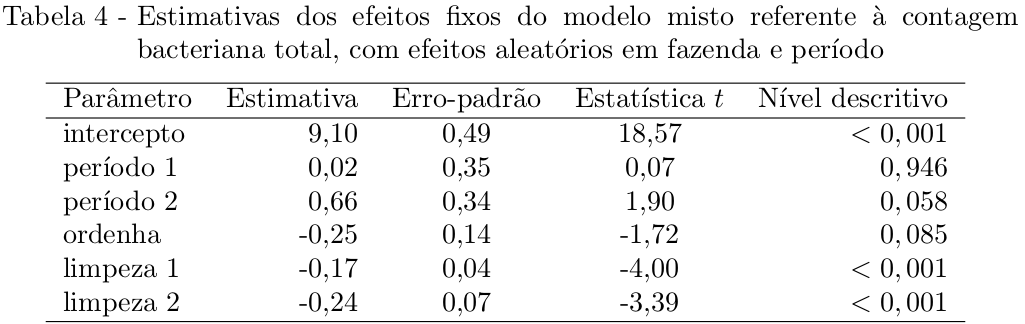
\includegraphics[scale=0.29]{long_tab04.png}
            %\caption{}
            \label{Rotulo}
        \end{figure}
\end{frame}


\begin{frame}{Modelo Ajustado - Interpretação}
    \begin{itemize}
      \item Efeito de limpeza foram estatisticamente significativo
      \item O efeito de perı́odo 2 foi siginificativo 
      \item Dado a presença do efeito aleatório em fazenda, pode-se pensar em
  nı́veis de contaminação individuais

    \end{itemize}
\end{frame}

\begin{frame}{Modelo Marginal - Regressão Logística}
    \begin{itemize}
      \item Explicar probabilidade da fazenda estar com CBT dentro dos limites aceitáveis  
      \item Selecionado a estrutura de correlação AR-1
    \end{itemize}
      \begin{figure}[!h]
            \centering
            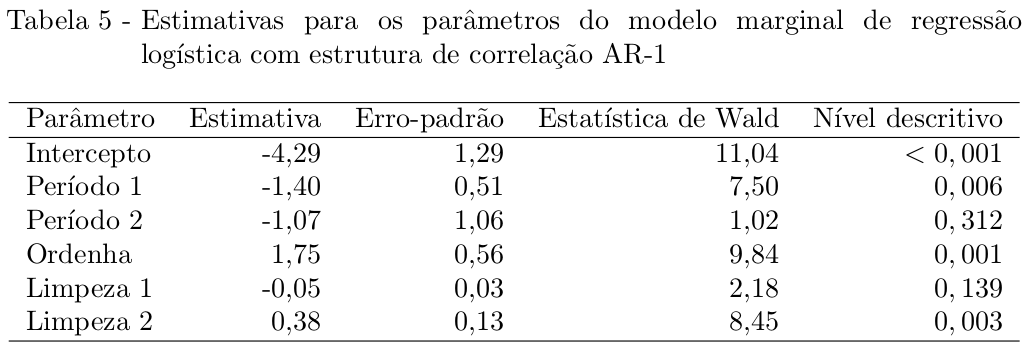
\includegraphics[scale=0.29]{long_tab05.png}
            %\caption{}
            \label{Rotulo}
    \end{figure}
    
\end{frame}


\begin{frame}{Modelo Misto - Regressão Logística}
    \begin{block}{}
        \eta_i_t = ln(\frac{\pi_i_t}{1-\pi_i_t}) = (\beta_0 + b_i_0) + \beta_1limp1 + \beta_2limp2
    \end{block}

      \begin{figure}[!h]
            \centering
            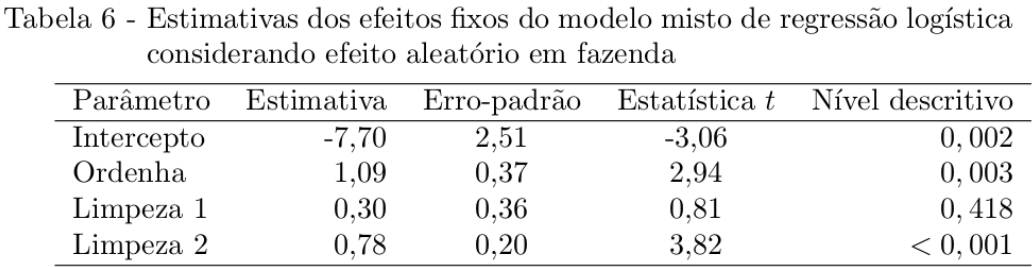
\includegraphics[scale=0.29]{long_tab06.png}
            %\caption{}
            \label{Rotulo}
    \end{figure}
    
\end{frame}

\begin{frame}{Regressão Logística}
    \begin{itemize}
      \item Não considera o efeito de período
      \item Resultado similar ao modelos anteriores
      \item Estima mais um parâmetro de variância do efeito aleatório na fazenda 
      \item Capta a heterogeneidade entre as fazendas
    \end{itemize}

\end{frame}



\subsection{Considerações Finais}

\begin{frame}{Considerações Finais}
    \begin{itemize}
      \item As duas abordagens destacam a importância da adequação dos procedimentos
      \item Constata-se que que as propriedades precisam de melhorias nos processos de manejo.
      \item Variável reposta com distribuição Poisson
        \begin{itemize}  
          \item Pode ocorrer superdisperção
          \item Heterogeneidade entre as propriedades
        \end{itemize}
      \item Modelo marginal: 
        \begin{itemize}  
          \item Inferir sobre o BTC médio
          \item Período não relevante
          \item Limpeza 1 e ordenha altamente relevante
        \end{itemize}
      \item Modelo misto: 
        \begin{itemize}  
          \item Hipóteses envolvendo parâmetros individuais
        \end{itemize}

          
      


    \end{itemize}

\end{frame}


    
    

\begin{frame}
    \Huge{\centerline{Obrigado pela atenção!!}}
\end{frame}

\end{document}


